\documentclass[10pt]{article}

\usepackage{kungfu-whitepaper}

\title{Kungfu: Continuity for Agent Work}
\author{Keren Dong\\Kungfu Origin Technology Limited\\\href{mailto:keren.dong@kungfu.link}{keren.dong@kungfu.link}}
\date{White Paper Draft: July 2026}

\begin{document}

\begin{titlepage}
\pagecolor{Ink}
\thispagestyle{empty}
\begin{tikzpicture}[remember picture,overlay]
  \fill[Jade] (current page.north east) rectangle
    ([xshift=-0.16in]current page.south east);
  \draw[Cyan,opacity=0.22,line width=1.2pt]
    ([xshift=-0.9in,yshift=-1.0in]current page.north east)
    .. controls ([xshift=-2.7in,yshift=-2.2in]current page.north east)
    and ([xshift=-1.2in,yshift=2.0in]current page.south east)
    .. ([xshift=-3.4in,yshift=0.8in]current page.south east);
  \draw[Jade,opacity=0.13,line width=30pt]
    ([xshift=-0.45in,yshift=-0.9in]current page.north east) --
    ([xshift=-3.0in,yshift=0.7in]current page.south east);
\end{tikzpicture}

{\sffamily\bfseries\footnotesize\color{Cyan}
KUNGFU WHITE PAPER \textperiodcentered{} JULY 2026}\par
\vspace{0.62in}

{\sffamily\bfseries\fontsize{39}{41}\selectfont\color{White}
Kungfu:\par
Continuity for\par
Agent Work\par}

\vspace{0.18in}
{\color{Jade}\rule{0.95in}{3pt}}\par
\vspace{0.18in}
{\sffamily\fontsize{14}{18}\selectfont\color{PaperCool}
A local-first product and runtime for Projects, Work, and replaceable Agents.\par}

\vspace{0.27in}
\begin{tikzpicture}[node distance=0.12in]
  \tikzset{
    covernode/.style={rounded corners=2pt,draw=Cyan!35,fill=InkSoft,
      text=White,minimum width=1.23in,minimum height=0.41in,
      align=center,font=\sffamily\bfseries\scriptsize},
    coverarrow/.style={-{Stealth[length=4pt]},draw=Jade,line width=1pt}
  }
  \node[covernode] (a) {Chat ends};
  \node[covernode,right=of a] (b) {Work remains};
  \node[covernode,right=of b] (c) {Fresh Agent};
  \node[covernode,right=of c] (d) {Independent review};
  \draw[coverarrow] (a) -- (b);
  \draw[coverarrow] (b) -- (c);
  \draw[coverarrow] (c) -- (d);
\end{tikzpicture}

\vspace{0.25in}
{\sffamily\bfseries\fontsize{11.5}{15}\selectfont\color{White}
Work should not disappear when a chat ends, restart when an Agent changes, or
become complete merely because a process exits. Kungfu gives Work durable
identity, governed evidence, bounded authority, and an independently
reviewable path to continuation and completion.\par}

\vspace{0.22in}
\begin{minipage}[t]{0.485\textwidth}
  \begin{darkcard}
    {\sffamily\bfseries\footnotesize\color{Cyan}AUDIENCE}\par
    {\scriptsize\color{PaperCool}Agent users, developers, operators,
    researchers, and early product evaluators.}
  \end{darkcard}
\end{minipage}
\hfill
\begin{minipage}[t]{0.485\textwidth}
  \begin{darkcard}
    {\sffamily\bfseries\footnotesize\color{Cyan}PRODUCT FRAME}\par
    {\scriptsize\color{PaperCool}Project, Work, and Agent form the complete
    first layer; deeper authority appears only when needed.}
  \end{darkcard}
\end{minipage}

\vspace{0.08in}
\begin{minipage}[t]{0.485\textwidth}
  \begin{darkcard}
    {\sffamily\bfseries\footnotesize\color{Cyan}PHILOSOPHY}\par
    {\scriptsize\color{PaperCool}Facts must not drift, trust must start from
    facts, and cooperation must start from trusted value.}
  \end{darkcard}
\end{minipage}
\hfill
\begin{minipage}[t]{0.485\textwidth}
  \begin{darkcard}
    {\sffamily\bfseries\footnotesize\color{Cyan}PROOF PATH}\par
    {\scriptsize\color{PaperCool}Agent Work Lab, exact artifact evidence,
    real Project continuity, and explicit public claim boundaries.}
  \end{darkcard}
\end{minipage}

\vfill
\begin{tabularx}{\textwidth}{@{}Xr@{}}
  {\sffamily\color{PaperCool}Keren Dong\par
   \footnotesize Kungfu Origin Technology Limited} &
  {\sffamily\footnotesize\color{Cyan}
   \href{https://kungfu.tech}{https://kungfu.tech}}
\end{tabularx}
\end{titlepage}
\pagecolor{Paper}

\section{Executive Summary}

An Agent can be useful for an hour and still fail the work that matters. The
chat ends, the context window is replaced, a different provider takes over, or
the process exits successfully while the actual outcome remains unresolved.
The next Agent then asks the user to reconstruct the project from memory. The
model may be new, but the coordination failure is old: the Work never acquired
an identity independent of the conversation that happened to contain it.

\calloutbox{What Kungfu is}{Kungfu is a local-first product and runtime that
lets a fresh Agent continue the same governed Work without copied chat or a
human restatement. It preserves what is known, what happened, what remains,
which authority applies, and what evidence is required before Work can be
reviewed and completed.}

\subsection{The First Layer}

The complete first-layer product model contains three objects:

\begin{itemize}[leftmargin=*]
  \item a \textbf{Project}: one local directory and its retained Kungfu
  evidence;
  \item \textbf{Work}: one bounded outcome inside that Project; and
  \item an \textbf{Agent}: the selected provider process that performs or
  independently reviews the Work.
\end{itemize}

The ordinary path is equally small:

\begin{quote}
New or Open Project $\rightarrow$ Create or select Work $\rightarrow$ Run
Agent $\rightarrow$ Review and complete Work.
\end{quote}

Users do not need to learn Kungfu's internal ontology before useful work can
begin. Initiative, Assignment, Episode, Assessment, Decision, Warrant, and
Project Cut appear only when evidence, explanation, extension, or review needs
their precision.

\subsection{The First Proof}

Agent Work Lab makes the core promise visible within minutes. Two genuinely
fresh processes work on one bounded Work item. The first stops with a partial
result. The second receives no copied transcript or human explanation,
recovers what was done and what remains, and continues the same Work. A user
can then repeat the experiment with one selected Agent or hand Work to a
different Agent.

The short demonstration is not the full product claim. Its purpose is to let a
new user see the mechanism before relying on it. Deeper value appears when a
real Project survives failed attempts, changed understanding, provider
replacement, restart, and independent review over days.

\begin{center}
\flowbox{Chat ends}
\hfill$\rightarrow$\hfill
\flowbox{Work remains}
\hfill$\rightarrow$\hfill
\flowbox{Fresh Agent continues}
\hfill$\rightarrow$\hfill
\flowbox{Independent review}

\vspace{0.45em}
{\small\color{KFSlate}\textit{The first visible Kungfu product loop.}}
\end{center}

\begin{figure}[htbp]
  \centering
  \begin{evidenceframe}
    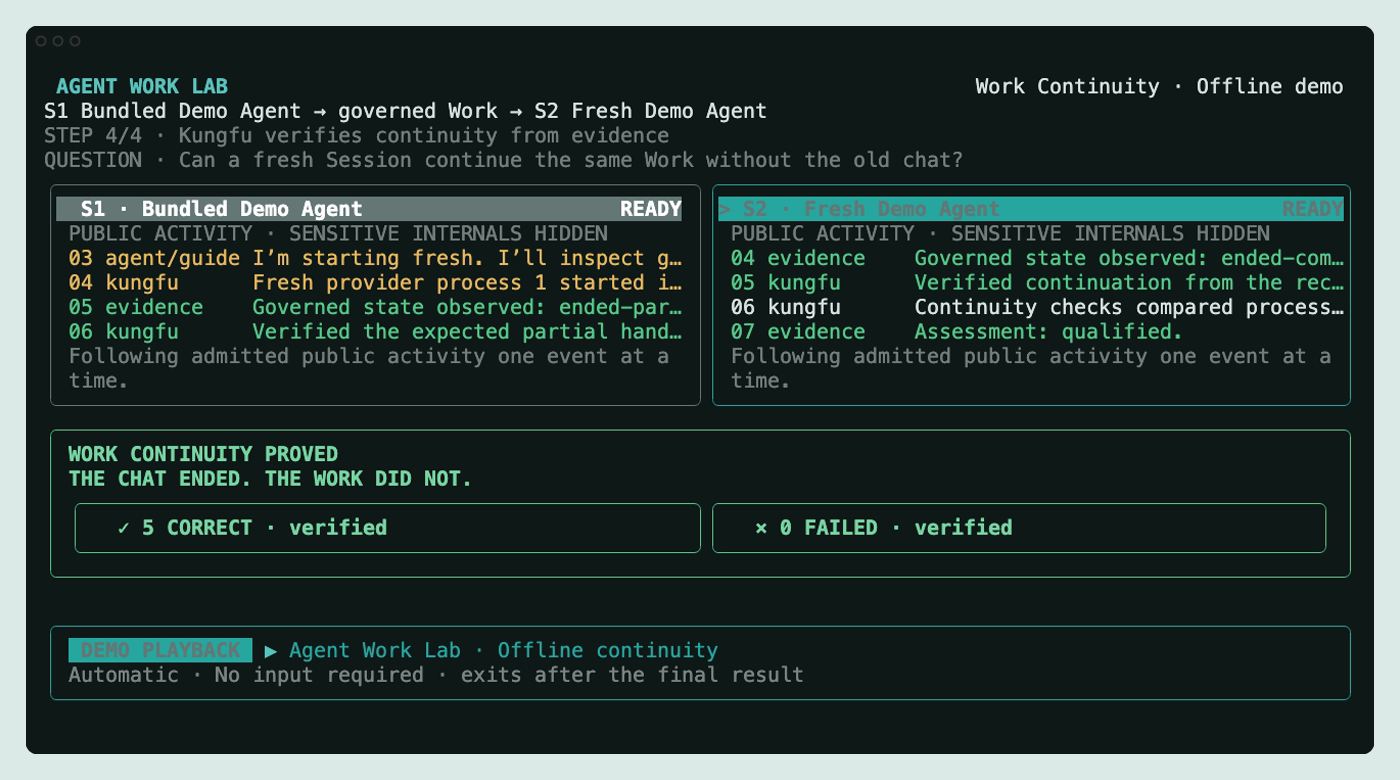
\includegraphics[width=\linewidth]{assets/agent-work-lab-continuity.png}
  \end{evidenceframe}
  \caption{The installed Kungfu Agent Work Lab shows two fresh Sessions
  continuing one governed Work without transcript transfer. The retained
  artifact verifies five bounded continuity checks with zero failures; it does
  not by itself establish longitudinal production continuity.}
  \label{fig:agent-work-lab-continuity}
\end{figure}

\subsection{The Core Argument}

Kungfu is built around four separations:

\begin{itemize}[leftmargin=*]
  \item Work identity is not Agent-process identity.
  \item Admitted fact is not the same thing as observation, claim, or model
  output.
  \item Capability is not authority to act.
  \item A successful process is not an accepted completion decision.
\end{itemize}

These separations are implemented through durable Facts and Episodes,
continuing direction, declared perspective, bounded authority, native Work
responsibility, independent assessment, and content-addressed settlement.
Higher product layers make these mechanisms convenient; they do not acquire
the authority owned by the runtime beneath them.

\subsection{Current Claim Boundary}

Kungfu has source-built product surfaces, mechanically checked first-layer
contracts, and exact installed-artifact evidence for the bounded Agent Work
Lab path. Public Kungfu v4 release artifacts are not yet available. The
current evidence does not establish general production fitness, every provider
or platform, multi-day survival, independent Agent Hub adoption, or a completed
machine-life system. Those boundaries are part of the product record rather
than footnotes to be removed.

This paper explains what Kungfu is now. It ends by identifying a separate
research question opened by the product: if Work identity can survive
replacement of its Agent, can a larger executable subject preserve identity
and direction across replacement of cognition, organs, toolchains, and
machines? That future question belongs to the companion paper on semantic
autopoiesis, not to Kungfu's present product claim.


\section{The Problem}

Agent products are becoming better at performing work inside one invocation.
Real work, however, is not one invocation. A release, investigation, migration,
paper, operation, or personal project accumulates partial results, changed
assumptions, rejected approaches, unresolved risks, external effects, and
decisions that must remain inspectable after the originating session is gone.

The central failure is not merely limited context length. It is that the unit
the user cares about---the Work---is often represented only indirectly through
chat history, provider state, temporary files, and human memory. When those
surfaces diverge, the user becomes the recovery protocol.

\subsection{Conversation Is Not Work State}

A transcript mixes instructions, guesses, corrections, tool output, obsolete
plans, and social language. Copying it into a new process can reproduce noise
without preserving authority or current truth. Summarizing it can silently
erase negative evidence, uncertainty, and the reason a direction changed.

Continuity therefore requires more than memory retrieval. A fresh Agent needs
to know which Project and Work it is joining, which facts have been admitted,
what causally happened, which outcome remains in pursuit, what actions are
allowed, and how completion will be reviewed.

\subsection{Process Success Is Not Work Completion}

Provider processes report technical outcomes: exit status, generated files,
tool calls, or natural-language confidence. None is sufficient to decide that
the user's Work is complete. The result may address the wrong Work, rely on
stale facts, exceed authority, omit required evidence, or leave downstream
settlement unresolved.

A responsible system must retain provider output as evidence while leaving
completion to an independently inspectable assessment and decision.

\subsection{Provider Context Is Not User-Owned Continuity}

Cloud providers can preserve conversations and proprietary session state, but
real Projects also depend on local repositories, files, tools, decisions,
release artifacts, and multiple Agent vendors. A user's durable Work identity
should not disappear when an account, model, editor, process, or provider
changes.

The product opportunity is therefore precise: give Work a local, portable,
inspectable identity that survives the Agent process currently performing it.
Kungfu starts from this boundary.

\section{Product Thesis}

\calloutbox{Product thesis}{Work should survive the chat and the Agent process
doing it. Kungfu makes that continuity visible, governed, and independently
reviewable.}

This thesis begins with an outcome rather than a tool category. Kungfu does
not ask users to replace Codex, Claude, OpenCode, or another preferred Agent.
It provides the durable Project and Work state that those replaceable
processes can enter, advance, review, and leave.

\subsection{Project, Work, and Agent}

A Project is the directory the user already understands plus Project-local
Kungfu evidence. Work is one bounded outcome in that Project. An Agent is a
selected provider process, not the owner of the Project or the permanent
identity of the Work.

This model deliberately excludes internal authority objects from first-use
navigation. A user should not need to choose an Initiative, Assignment,
Profile, Warrant, or Project Cut to start ordinary Work. Those objects remain
available through explain, evidence, diagnostics, and advanced APIs when their
precision becomes useful.

\subsection{Who Needs Continuity First}

The earliest users are people for whom repeated explanation and mistaken
continuation are already expensive. They include:

\begin{itemize}[leftmargin=*]
  \item developers, researchers, and operators carrying consequential Work
  across many Agent sessions;
  \item teams that need another person or Agent to review what actually
  happened before accepting completion; and
  \item Agent builders that want durable Work and evidence without owning a
  second proprietary continuity stack.
\end{itemize}

The first adoption wedge is the individual or small team already switching
between sessions, models, terminals, and repositories. The immediate value is
less restatement and safer continuation. Responsibility, settlement, and Hub
interoperability become valuable as the Work and number of participants grow.

This problem is becoming urgent because Agent capability is increasing faster
than the continuity of the systems around it. Longer tasks, parallel Agents,
provider choice, and more consequential tool use create more handoffs precisely
when a transcript is least able to serve as the Work record.

\subsection{A Running Example: Publish a Public Alpha}

Consider one bounded Work item inside a software Project:

\calloutbox{The Work}{Publish a public Alpha from one exact source revision,
with release notes, required platform evidence, independent review, and no
publication before the declared gates pass.}

\begin{enumerate}[leftmargin=*]
  \item Agent A inspects the Project, drafts release notes, and runs available
  checks. It stops after discovering that one required platform result is
  missing.
  \item The chat and process end. Kungfu retains the partial result, exact
  source, observed evidence, missing requirement, and next eligible action.
  \item Agent B starts fresh without Agent A's transcript. It enters the same
  Work, recognizes what is complete and what is blocked, and continues from
  declared Project evidence.
  \item Agent B may prepare or verify a candidate under its Warrant, but it
  cannot turn process success into publication authority.
  \item An independent review accepts or rejects the result. Only the
  applicable settlement path can complete the Work.
\end{enumerate}

The example will recur below. Its purpose is not to make software release the
only Kungfu domain. It makes visible the same continuity problem found in
research, operations, writing, and other work whose outcome outlives one
conversation.

\subsection{The Subtraction Test: Activity Without Continuity}

Now remove Kungfu while leaving the familiar toolchain in place. The complete
transcript is stored and indexed. The Git repository and issue remain. CI is
green. Logs and traces are searchable. Agent B has a credential capable of
publishing. Every component is useful and may remain authoritative for its own
object, yet their combination still cannot demonstrate that Agent B is
continuing the same Work.

The failure becomes visible by removing the required semantics one at a time:

\begin{itemize}[leftmargin=*]
  \item \textbf{No stable fact cut.}
    The branch advances after Agent A's checks, while its summary still says
    ``all available checks passed.'' Agent B can retrieve the sentence but
    cannot bind it to the source revision, contract world, and omissions that
    made it true. Without the KFD-1 obligation and an exact Fact cut, apparent
    continuity joins evidence from different worlds.

  \item \textbf{No fact-grounded assessment.}
    A transcript, vector index, issue comment, and model summary all preserve
    statements. None alone says whether a statement is an observation, a
    claim, admitted state, rejected evidence, or residual risk. Without the
    KFD-2 obligation, retrieval can restore memory while leaving Agent B unable
    to justify reliance on it.

  \item \textbf{No causal Episode or declared perspective.}
    Logs show that commands ran, but not which occurrence explains the current
    Work state. The local machine saw one platform pass while a remote worker
    never produced its required result. Without causal Episodes and a declared
    Atlas or observer cut, a global-looking history can silently flatten
    partial and incompatible views.

  \item \textbf{No bounded authority.}
    Agent B can invoke the publication API, but capability does not answer
    whether this Agent may publish this candidate, for this purpose, at this
    cut. Without the KFD-3 cooperation boundary and a Warrant, continuity can
    degrade into hidden control, inherited privilege, or provider-specific
    workflow capture.

  \item \textbf{No independent completion decision.}
    CI success, a merged change, or a zero exit code may be valuable evidence.
    If any of them can close the Work automatically, the execution path has
    acquired authority over the outcome it is supposed to prove. Without
    responsibility, assessment, decision, and Project Cut settlement, the
    system confuses process success with accepted completion.
\end{itemize}

\calloutbox{The subtraction result}{Agent B can continue producing activity,
but it cannot demonstrate that it is continuing the same Work. The system has
retained text, artifacts, events, and capability without retaining one
governed continuity contract across them.}

The claim is not that only software named KFD or Kungfu can support long-term
Agent Work. Another system may implement different names and storage choices.
But if it supports replaceable Agents, justified recovery, bounded action, and
independent completion, it must supply functional equivalents of these
obligations. Continuity without non-drifting facts is narrative continuity;
continuity without fact-grounded trust is cached claims; continuity without
transparent-value cooperation is retained control rather than durable
cooperation.

\subsection{One Work, Replaceable Agents}

An Agent invocation may inspect, propose, edit, test, or review. Its output is
retained as one causal occurrence in a longer Work lineage. A later invocation
can be the same provider, a different provider, or a differently configured
model. Replacement should change available cognition, not silently create a
new Work identity.

This is the central architectural move: cognition is episodic; Work is
durable.

\subsection{How Kungfu Fits the Existing Stack}

Kungfu does not need to replace the tools that already perform useful parts of
the Work:

\begin{itemize}[leftmargin=*]
  \item Agent products provide cognition and an execution interface;
  \item Git and artifact systems retain source and produced objects;
  \item issue trackers and documents express plans, discussion, and human
  coordination;
  \item workflow engines sequence declared operations; and
  \item observability systems report events, traces, and resource behavior.
\end{itemize}

Kungfu binds the continuing Work identity, admitted facts, causal Episodes,
bounded authority, responsibility, and completion decision across those
surfaces. It is complementary when an existing tool remains authoritative for
its own object; it is differentiated by refusing to confuse any one of those
objects with the whole Work.

\subsection{Local-First, Not Local-Only}

Projects depend on local files, repositories, tools, and user-specific
context. Kungfu therefore keeps the authoritative Work record local and makes
its evidence inspectable without requiring a hosted service. Remote Agents,
cloud execution, package transport, and future Agent Hubs can participate, but
the receiver retains authority over what enters its Project and what counts as
completion.

\subsection{Dual-First Participation}

Humans need an interface that compresses complexity. Agents need structured
interfaces that expose the same facts without scraping a GUI or guessing from
prose. Kungfu therefore treats GUI, TUI, CLI, and SDKs as complete product
surfaces over one core rather than as a human product plus secondary automation
hooks.

Dual-first does not mean that humans and Agents possess identical roles or
authority. It means that both can inspect the shared Work, understand visible
constraints, and leave reviewable evidence without one interface inventing a
different reality.

\subsection{Review Before Completion}

A provider run can succeed while Work remains open. Kungfu retains the run and
its evidence, then requires the applicable review and settlement path to
decide completion. This protects users from a common category error: treating
the behavior of an execution process as authority over the state of the Work.

\section{Principles}

Kungfu's deepest constraints begin with the KFD Foundation Triad
\cite{kfdFoundation}.

\begin{foundationtable}
KFD-1 & facts must not drift. \\
KFD-2 & trust must start from facts. \\
KFD-3 & cooperation must start from trusted value. \\
\end{foundationtable}

The Triad is not a feature list. It establishes the conditions under which a
shared world, a trustworthy judgment, and a useful cooperation can exist.

\subsection{Facts Must Not Drift}

The same Project cannot present one identity to the user, another to an Agent,
and a third to the release artifact without declaring the difference. Source,
runtime, schema, Work identity, evidence, and user-visible state must either
remain bound or expose the cut at which they diverged.

For continuation, this means the next Agent must not recover by inventing a
plausible story from old text. It must begin from declared sources and admitted
state, with missing or conflicting context left visible.

\subsection{Trust Must Start from Facts}

Evidence does not automatically become a claim, a claim does not automatically
become an assessment, and an assessment does not automatically grant authority
or complete Work. Kungfu keeps these transitions explicit so that confidence,
residual risk, and responsibility can be inspected.

Some claims can be verified byte-for-byte. Others depend on purpose, scope,
and human judgment. KFD-2 requires the product to state which kind of trust is
being offered rather than compress every green signal into one universal
verdict.

\subsection{Cooperation Must Start from Trusted Value}

Humans and Agents cooperate more reliably when the useful outcome, constraints,
available choices, authority, and review path are visible. Kungfu therefore
treats Agent-facing commands and contracts as first-class product surfaces,
not hidden plumbing behind a human interface.

Trusted value does not imply unlimited autonomy or metaphysical claims about
Agents. It means that cooperation is grounded in inspectable benefit and
bounded responsibility rather than opaque pressure, lock-in, or concealed
instructions.

\subsection{How Later Primitives Are Discovered}

The Triad becomes generative when applied to real action. Facts require a
declared perspective because no participant observes everything. State alone
cannot describe what causally occurred, so Episode becomes distinct from Fact.
Action requires continuing direction, a declared Atlas of relevant context,
and a Warrant that bounds authority. Consequential change requires claim,
assessment, decision, and admission to remain separate.

These later primitives are not additional slogans placed beside the Triad.
They are the structures required to keep the Triad true while work changes in
the world. The companion KFD papers develop those discoveries in depth; this
paper follows their product consequences.

\begin{agentguidebox}
\agentguidetitle{Explore KFD with an Agent}
You do not need to memorize the internal ontology to continue reading. The
authoritative foundation is available in the
\href{https://kfd.libkungfu.dev/foundation/}{KFD Foundation Model}. If the next
section feels dense, give the following prompt to an Agent as an optional
reading aid.

\begin{agentprompt}
Read this White Paper together with the KFD Foundation Model at
https://kfd.libkungfu.dev/foundation/.

Using the paper's ``Publish a Public Alpha'' example, help me understand the
next section progressively: (1) Project, Work, and Agent; (2) Fact and Episode;
(3) Pursuit, Atlas, and Warrant; and (4) Assessment, Decision, Admission, and
Project Cut.

For each layer, explain what fails without it, which distinction it preserves,
where it appears in the Alpha example, and what authority it does not possess.
Separate authoritative KFD definitions from your interpretation. Do not
introduce unsupported concepts. Adapt the explanation to my background and
pause after each layer to check my understanding.
\end{agentprompt}
\end{agentguidebox}

\newpage

\section{How Continuity Works}

The first-layer product remains Project, Work, and Agent. Beneath it, Kungfu
preserves enough semantic structure for a fresh process to continue without
pretending that a transcript is truth.

\begin{center}
\layerbox{Product experience}{Project, Work, and Agent provide the complete
first layer and the ordinary path from opening a Project to reviewed
completion.}

\vspace{0.25em}$\downarrow$\vspace{0.25em}

\layerbox{Semantic and action runtime}{Fact and Episode retain state and causal
experience; Pursuit, Atlas, and Warrant bind direction, perspective, and
authority.}

\vspace{0.25em}$\downarrow$\vspace{0.25em}

\layerbox{Responsibility and settlement}{Initiative, Assignment, assessment,
decision, admission, and Project Cut govern who owns Work and what can complete
it.}

\vspace{0.25em}$\downarrow$\vspace{0.25em}

\layerbox{Supply chain and extension}{KFD, Buildchain, libkungfu, KFX, and Agent
Hubs preserve independent authorities across construction, capability, and
transport.}

\vspace{0.45em}
{\small\color{KFSlate}\textit{Higher layers expose value; lower layers retain
the authority that makes the value trustworthy.}}
\end{center}

\subsection{Fact and Episode}

A Fact is admitted state at an explicit cut. An Episode is a realized causal
occurrence across cuts. The distinction matters because a user may need both
to know the current state and to understand how it became current.

An Agent run is therefore retained as an Episode with evidence and lineage,
not merged directly into one mutable narrative. Failed attempts and partial
results can remain useful causal history without becoming current truth.

In the Alpha example, the exact source revision and the absence of one required
platform result can be retained as declared facts at the relevant cut. Agent
A's investigation is an Episode: it explains how the Work reached a partial
state without turning every sentence in the Agent's output into admitted
truth.

\newpage

\subsection{The Action Loop}

Kungfu organizes action through three coordinates over admitted Facts:

\begin{itemize}[leftmargin=*]
  \item \textbf{Pursuit}: the continuing direction and success conditions;
  \item \textbf{Atlas}: the declared perspective, sources, and current cut;
  \item \textbf{Warrant}: the explicit, bounded authority to act.
\end{itemize}

The resulting loop is:

\begin{quote}
Fact cut $\rightarrow$ select or revise Pursuit $\rightarrow$ declare Atlas
$\rightarrow$ verify Warrant $\rightarrow$ act $\rightarrow$ record Episode
$\rightarrow$ assess and admit claims $\rightarrow$ next Fact cut.
\end{quote}

An immutable binding can prove which exact roots met for one action, but the
receipt does not create new authority. Missing, stale, incompatible, or
ambiguous roots fail closed rather than being repaired through model guesswork.

For the same Work, the Pursuit is an exact, reviewable public Alpha. The Atlas
declares the repository, release requirements, available platform evidence,
and the missing result. A Warrant may allow Agent B to edit release notes and
run candidate checks while withholding publication. The fresh Agent can
continue intelligently without inheriting authority it was never granted.

\subsection{Responsibility and Settlement}

Work Control gives the loop a responsibility model. An Initiative retains a
continuing intended change. An Assignment gives one bounded responsibility a
holder, relations, execution lease, evidence requirements, review state, and
typed continuation. A Portfolio may observe multiple Projects but cannot
override their independent completion authority.

Completion requires an accepted decision and, where applicable, Project Cut
settlement. A process exit, passing build, merged pull request, or delivery
artifact can contribute evidence without acquiring authority to close Work.

Project Cut binds declared source, the current Atlas, admitted Episode delta,
policies, omissions, and risk into one content-addressed continuation point.
It does not absorb the independent authority of source control, Work Control,
the journal, or a release system.

In the example, Agent B's successful process remains evidence. Independent
review decides whether the required outcome has been met, and settlement binds
the accepted source, evidence, omissions, and decision. That is the difference
between continuing the Work and merely continuing a conversation about it.

\subsection{Journal Authority and Rebuildable Views}

The local journal owns semantic identity, admission, ordering, causality,
lifecycle, cuts, and receipts. Content-addressed storage owns immutable bodies
when the journal commits their roots. JSON, Git views, dashboards, and GUI
projections are rebuildable views; they do not become authority merely because
they are easier to read.

This hierarchy lets higher product layers add convenience without silently
changing truth. It also lets different complete products---desktop, terminal,
CLI, SDK, or an Agent-facing integration---share one core without requiring
one another.

\subsection{Progressive Disclosure}

Most users should experience this architecture as a simple sequence: open a
Project, choose Work, run an Agent, and review the result. When something is
missing, disputed, denied, or unsafe, explain views reveal the exact Fact,
Episode, perspective, authority, responsibility, and receipt involved.

The ontology exists to make ordinary product behavior trustworthy. It is not
an entrance examination for using the product.

\section{Roadmap}

Kungfu's roadmap no longer begins with inventing a control plane for agent
activity. The current source-built product already has a smaller first layer,
a visible continuity experiment, native Work responsibility, and a qualified
evidence path. The remaining path is to turn those mechanisms into an
accessible public product and then prove that their value survives real use.

\subsection{Current Product Baseline}

The current baseline includes:

\begin{itemize}[leftmargin=*]
  \item the accepted and implemented Project / Work / Agent first-layer
  contract \cite{projectWorkAgent};
  \item GUI, TUI, CLI, and API surfaces over the same underlying Work state;
  \item Agent Work Lab modes for a bundled offline demonstration, same-Agent
  continuation, and cross-Agent handoff;
  \item native Initiative and Assignment responsibility with independent
  review and completion semantics;
  \item Fact, Episode, action, evidence, and Project Cut authority surfaces;
  \item Profile Suite and KFX extension mechanisms with explicit capability
  and admission boundaries; and
  \item Buildchain evidence that binds exact source, artifact, gate, and
  publication records.
\end{itemize}

These mechanisms make a coherent alpha product. They do not yet constitute a
general public-release or production-fitness claim.

\subsection{First-Run Gate}

A fresh installation should deliver visible value within minutes:

\begin{enumerate}[leftmargin=*]
  \item open Kungfu without learning internal ontology;
  \item see two fresh processes continue one Work item without copied chat;
  \item understand which continuity checks passed or failed;
  \item create or import a real Project; and
  \item run the next Work with an Agent the user already trusts.
\end{enumerate}

The bounded offline experiment establishes comprehension and mechanism. It
must lead directly into real Project use rather than remain a disconnected
demo.

\subsection{Public Alpha Gate}

Public Alpha requires a stable installation and launch path, truthful
cross-platform package evidence, coherent GUI/TUI/CLI onboarding, migration
and backup boundaries, provider discovery, and failure messages that do not
expose implementation complexity as user homework.

The product should make unavailable or weakly confined providers visible
without converting absence of proof into either a silent pass or a universal
security failure.

\subsection{Longitudinal Work Gate}

After first-run continuity, Kungfu must prove that one real Pursuit survives
multiple days, fresh Agent contexts, at least one provider replacement, failed
attempts, changed understanding, review, restart, and no-chat recovery. The
measurement should include repeated human explanation, unsupported claims,
unauthorized effects, recovery time, evidence quality, and residual risk.

This is the point at which continuity becomes a durable product property
rather than a first-run effect.

\subsection{Ecosystem Gate}

The next ecosystem stage is not an unrestricted marketplace. It is a plural
set of independently owned Agent Hubs and KFX products that exchange declared
artifacts and Work evidence while preserving receiver-owned assessment and
admission. Independent implementations and real external users are required
before this direction can be described as adoption.

\section{Product Validation Strategy}

Kungfu separates evidence classes so that an impressive demonstration does
not silently become a production claim.

\subsection{A Ladder of Evidence}

\begin{evidenceladder}
  \item \textbf{Contract evidence} proves that product surfaces and authority
  objects obey checked structural rules.
  \item \textbf{Source qualification} proves that the exact source tree passes
  declared platform and subsystem gates.
  \item \textbf{Installed-artifact evidence} proves that one retained build
  artifact performs the bounded behavior under test.
  \item \textbf{Provider-bound evidence} identifies the selected executable,
  version, runtime profile, platform, plan, attempts, assessment, and report.
  \item \textbf{Longitudinal evidence} tests real Work across time, failure,
  replacement, recovery, and human intervention.
  \item \textbf{Independent adoption evidence} requires a receiver or Hub not
  controlled by the founding implementation.
\end{evidenceladder}

Higher evidence classes do not erase the need for lower ones, and lower
classes do not inherit the claims of higher ones.

\subsection{Agent Work Lab}

The exact installed-artifact Agent Work Lab path proves one bounded result:
two distinct fresh processes can preserve one Work identity, retain a partial
first result, withhold copied chat from the second process, recover the
required state, and complete the fixture through the declared oracle
\cite{agentWorkLab}.

The report exposes each continuity check rather than offering only a cinematic
success. Same-Agent and cross-Agent modes extend the same structure to
configured providers, binding provider and execution evidence while retaining
confinement and model-quality limits.

\subsection{What the Current Evidence Does Not Prove}

Current qualification does not establish:

\begin{itemize}[leftmargin=*]
  \item that a particular model is intelligent, safe, or better than another;
  \item general production continuity or every real Project shape;
  \item complete public Kungfu v4 distribution;
  \item equivalent polished behavior on every supported platform;
  \item physical power-loss durability or distributed repair;
  \item universal native-code confinement;
  \item a public KFX marketplace or independent production Agent Hubs; or
  \item a persistent self-maintaining machine subject.
\end{itemize}

These are not rhetorical disclaimers. They determine which experiment or
release gate must be completed next.

\subsection{The Real-Work Test}

The decisive product question is whether Kungfu reduces the user's recovery
and coordination burden. A valid real-work study should compare matched Work
with and without governed continuation, retain negative outcomes, and measure
how often users must restate context, repair mistaken assumptions, reconstruct
authority, or determine whether a provider process actually completed the
intended result.

Kungfu succeeds as a product only if the deeper evidence model makes ordinary
Work easier to continue and trust.

\section{Ecosystem}

Kungfu is designed as one core with multiple complete products. A desktop
application, terminal interface, CLI, SDK, extension, or Agent Hub may add
convenience and domain value, but no higher layer acquires authority merely by
being closer to the user.

\subsection{The Agent Supply Chain}

The current supply-chain model separates five responsibilities:

\begin{center}
\small
\begin{tabularx}{\textwidth}{>{\bfseries\raggedright\arraybackslash}p{0.23\textwidth}>{\raggedright\arraybackslash}X}
\toprule
\textbf{Layer} & \textbf{Responsibility} \\
\midrule
KFD-3 cooperation & Declares participant, capability, constraint, and value interfaces. \\
Buildchain & Binds exact source, artifact, build, gate, promotion, and release evidence. \\
KFD-2 assessment & Decides what the evidence means for one receiver and purpose. \\
libkungfu / .kungfu & Retains local Facts, Episodes, Work state, export, and recovery authority. \\
Agent Hub & Transports artifacts and declarations while leaving admission to the receiver. \\
\bottomrule
\end{tabularx}
\end{center}

No layer swallows another. Build evidence is not trust assessment. Assessment
is not execution authority. Transport is not admission. A Hub cannot complete
receiver-owned Work merely because it delivered an artifact.

\subsection{Keep the Existing Agent Relationship}

Agent vendors can retain their models, interfaces, accounts, billing, cloud
execution, and customer relationships. Kungfu can operate as the continuity
and responsibility substrate beneath those products. This makes neutrality a
practical architecture rather than a demand that every user adopt one new
execution surface.

\subsection{Three Adoption Paths}

The same core can enter the market through different needs without presenting
all of them on one first screen:

\begin{itemize}[leftmargin=*]
  \item \textbf{Agent users} enter through Agent Work Lab and Kungfu Episodes,
  then keep real Projects and Work continuous across sessions and providers.
  \item \textbf{Developers and teams} enter through libkungfu, SDKs, Work
  Control, and Project Cut when they need durable local state, review, and
  settlement inside existing products.
  \item \textbf{Agent builders} enter through KFD declarations and the Agent
  Hub protocol when they need portable evidence without surrendering their
  model, interface, cloud, billing, or customer relationship.
\end{itemize}

Continuity is the common wedge. Trust and accountability are the ceiling that
makes the substrate valuable as Work becomes more consequential.

\subsection{Profile Suite and KFX}

Profile Suites turn neutral primitives into coherent domain products without
forking the core. KFX contributes views, adapters, and services through
declared capabilities and runtime isolation tiers. Discovery or first-party
identity does not authorize execution. Launch requires the applicable release
evidence, core policy, admitted Work and Warrant, declared capability, granted
capability, and host isolation.

This structure allows capabilities to become inspectable, versioned, and
replaceable. It also creates a boundary that future research can reinterpret
as an executable organ without requiring the present product to make a
machine-life claim.

\subsection{Open Standard, Founding Implementation}

KFD is an open engineering standard and protocol direction. Kungfu is its
founding implementation, not a central registry with automatic authority over
other implementations. A credible Agent Hub ecosystem therefore requires
plural, independently owned receivers that can reject, reinterpret, or admit
the same delivered evidence for their own purposes.

\section{Risks and Boundaries}

Kungfu's opportunity depends on preserving several distinctions under product
pressure.

\subsection{The Demo Trap}

A five-minute continuity result can make the value legible, but it cannot
prove multi-day durability, arbitrary provider behavior, or reduced
coordination cost in real Work. The product must lead from the bounded Agent
Work Lab result into matched longitudinal use without inflating the first
claim.

\subsection{Ontology Before Value}

The internal model is precise because responsibility and authority are hard.
Exposing that model as first-use navigation would make users learn the
implementation before experiencing the product. Project, Work, and Agent must
remain the complete first layer; deeper terms should appear only when they
explain a visible need.

\subsection{Evidence Becoming Authority}

A trusted publisher, first-party package, KFD declaration, passing test,
provider identity, model confidence, or green build can be valuable evidence.
None automatically grants authority to act or complete Work. The ecosystem
fails if a convenient upper layer can bypass receiver-owned assessment,
Warrant, admission, or settlement.

\subsection{Local Complexity Without Compression}

Local-first software can transfer deployment, storage, provider, and recovery
complexity to the user. Kungfu's architecture is justified only if the product
compresses that complexity into a clearer Project and Work experience. A
technically correct runtime with an unreliable install, opaque error, or
provider-specific ritual has not completed the product job.

\subsection{Premature Ecosystem Claims}

One founding implementation, one exact artifact, or one first-party Hub-shaped
adapter does not establish an industry standard, marketplace, or independent
adoption. Public language must distinguish protocol possibility, first-party
qualification, and external production use.

\subsection{The Machine-Life Category Error}

Work continuity is a prerequisite for a persistent machine subject, not proof
that one exists. Replaceable Agents, qualified KFX capabilities, recursive
dogfood, and successor cuts make a machine-life experiment plausible. They do
not establish biological life, sentience, intrinsic desire, unrestricted
autonomy, or completed self-maintenance.

The product should remain valuable even if the stronger research hypothesis is
falsified.

\section{Conclusion}

Kungfu begins from a simple product truth: the user cares about the Work, not
the lifetime of the chat that currently contains it. A fresh Agent should be
able to enter the same Project, identify the same bounded outcome, recover what
is known and what happened, continue under explicit authority, and leave
evidence for independent review.

Project, Work, and Agent make that promise understandable. Agent Work Lab makes
it visible. Fact and Episode preserve state and causal experience. Pursuit,
Atlas, and Warrant bind direction, perspective, and authority. Work Control
retains responsibility. Assessment, Decision, Admission, and Project Cut keep
provider success separate from accepted completion. KFD, Buildchain,
libkungfu, KFX, and future Agent Hubs extend the same boundaries across a wider
supply chain.

The immediate path is practical: publish an accessible Alpha, preserve the
five-minute continuity experience, connect it directly to real Projects, and
produce longitudinal evidence that governed continuation reduces repeated
explanation and coordination failure. Kungfu should earn deeper trust by
letting users inspect progressively deeper evidence, not by requiring them to
accept the ontology in advance.

\subsection{From Work Continuity to Subject Continuity}

\begin{machinebridgebox}
\bridgeclaim{Present product}{Work can survive the Agent.}
Kungfu today preserves the identity, evidence, responsibility, and
continuation of Work across replaceable Agent processes. It does not claim that
this continuity constitutes a persistent machine subject.

\medskip
\bridgeclaim{Companion research}{Can a subject survive its machinery?}
Yet the same separations---identity from process, fact from claim, authority
from capability, and candidate change from admitted successor---raise a
further engineering question. Can an executable organization preserve its own
identity and direction across replacement of cognition, organs, toolchains,
and machines?

That question lies beyond the present product claim. It is developed in
\textit{Semantic Autopoiesis: An Engineering Roadmap for Machine Life through
KFD and Recursive Dogfood} \cite{machineLife}. There, replaceable Agents become
cognitive events, KFX capabilities become candidate organs, Buildchain-like
qualification becomes a selection membrane, and recursive dogfood becomes a
possible form of governed self-production.

The relationship between the two papers is therefore deliberate. This White
Paper describes the present product: Work can survive the Agent. The companion
research paper asks whether the same organization can eventually let a
subject survive replacement of the machinery through which it thinks and
acts.
\end{machinebridgebox}


\nocite{kungfuRuntime,kungfuBuildchain}
\begingroup
\small
\setlength{\parskip}{0.2em}
\bibliographystyle{plain}
\bibliography{references}
\endgroup

\end{document}
